\de{ĐỀ THI HỌC KỲ II NĂM HỌC 2022-2023}{THPT Chuyên Trần Đại Nghĩa}
\begin{center}
	\textbf{PHẦN 1 - TRẮC NGHIỆM}
\end{center}
\Opensolutionfile{ans}[ans/ans-THPTChuyen-TranDaiNghia]
%Câu1
\begin{ex}%[0T9Y3-1]%[Dự án đề kiểm tra HKII NH22-23- Phan Trung Hiếu]%[THPT Trần Đại Nghĩa]
	Trong các phương trình sau, phương trình nào là phương trình của một đường tròn?
	\choice
	{$5x^2+4y^2-x+4y-1=0$}
	{$x^2+y^2+2x-4y+9=0$}
	{\True $x^2+y^2-4x-2y+1=0$}
	{$x^2+y^2-6x+4y+13=0$}
	\loigiai{
	Ta có $a^2 + b^2 - c = 2^2 + 1^2 -1 = 4 > 0$ nên $x^2+y^2-4x-2y+1=0$ là phương trình của một đường tròn.
	}
\end{ex}
%Câu2
\begin{ex}%[0T8Y2-1]%[Dự án đề kiểm tra HKII NH22-23- Phan Trung Hiếu]%[THPT Trần Đại Nghĩa]
	Có bao nhiêu cách xếp $5$ học sinh thành một hàng dọc?
	\choice
	{$5$}
	{\True $5!$}
	{$4!$}
	{$5^5$}
	\loigiai{
		Xếp $5$ học sinh vào $5$ vị trí nên có tất cả $5!$ cách xếp.
	}
\end{ex}
%Câu3
\begin{ex}%[0T0Y1-2]%[Dự án đề kiểm tra HKII NH22-23- Phan Trung Hiếu]%[THPT Trần Đại Nghĩa]
	Một đội thanh niên tình nguyên gồm $12$ nam và $3$ nữ được phân công ngẫu nhiên về $3$ tỉnh, mỗi tỉnh $5$ người. Tính số phần tử của không gian mẫu
	\choice
	{$\mathrm{C}_{15}^5$}
	{$\mathrm{C}_{15}^5\cdot\mathrm{C}_{14}^3\cdot\mathrm{C}_{13}^5$}
	{$\mathrm{C}_{12}^4\cdot\mathrm{C}_3^1$}
	{\True $\mathrm{C}_{15}^5\cdot\mathrm{C}_{10}^5\cdot\mathrm{C}_5^5$}
	\loigiai{
		Có tất cả $15$ thanh niên tình nguyện.
		\begin{itemize}
			\item Bước 1: Chọn $5$ người trong $15$ người phân công về tỉnh thứ nhất.\\
			Có tất cả $\mathrm{C}_{15}^5$ cách chọn.
			\item Bước 2: Chọn $5$ người trong $10$ người còn lại phân công về tỉnh thứ hai.\\
			Có tất cả $\mathrm{C}_{10}^5$ cách chọn.
			\item Bước 3: Chọn $5$ người còn lại phân công về tỉnh thứ ba.\\
			Có tất cả $\mathrm{C}_5^5$ cách chọn.
		\end{itemize}
		Vậy số phần tử của không gian mẫu là $\mathrm{C}_{15}^5\cdot\mathrm{C}_{10}^5\cdot\mathrm{C}_5^5$.
	}
\end{ex}
%Câu4
\begin{ex}%[0T8Y1-1]%[Dự án đề kiểm tra HKII NH22-23- Phan Trung Hiếu]%[THPT Trần Đại Nghĩa]
	Một trường THPT, khối 10 có $280$ học sinh nam và $325$ học sinh nữ. Nhà trường cần chọn một học sinh ở khối 10 di dự dạ hội của học sinh thành phố. Hỏi nhà trường có bao nhiêu cách chọn?
	\choice
	{\True $605$}
	{$325$}
	{$280$}
	{$91000$}
	\loigiai{
		Có tất cả $280 + 325 = 605$ học sinh khối 10.
		Số cách chọn $1$ học sinh trong $605$ học sinh khối 10 đi dự dạ hội là $605$ cách chọn.
	}
\end{ex}
%Câu5
\begin{ex}%[0T0Y1-1]%[Dự án đề kiểm tra HKII NH22-23- Phan Trung Hiếu]%[THPT Trần Đại Nghĩa]
	Gieo một đồng tiền và một con xúc sắc. Số phần tử của không gian mẫu là
	\choice
	{$6$}
	{$8$}
	{\True $12$}
	{$24$}
	\loigiai{
		\begin{equation*}
			\Omega=\{(S,1),(S,2),(S,3),(S,4),(S,5),(S,6),(N,1),(N,2),(N,3),(S,4),(S,5),(N,6)\}.
		\end{equation*}
		Vậy $n(\Omega) = 2\cdot6=12$.
	}
\end{ex}
%Câu6
\begin{ex}%[0T9B3-1]%[Dự án đề kiểm tra HKII NH22-23- Phan Trung Hiếu]%[THPT Trần Đại Nghĩa]
	Cho phương trình $2x^2+2y^2-10x+12y+m=0$. Với giá trị nào của $m$ thì phương trình trên là phương trình đường tròn có bán kính $R=3$?
	\choice
	{$25$}
	{$\dfrac{25}{4}$}
	{\True $\dfrac{25}{2}$}
	{$\dfrac{4}{25}$}
	\loigiai{
		Phương trình trên tương đương $x^2 + y^2 -5x + 6y + \dfrac{m}{2}=0$.\\
		Ta có
		\begin{equation*}
			\left(\dfrac{5}{2}\right)^2 + (-3)^2 -\dfrac{m}{2} = 3^2\Leftrightarrow m = \dfrac{25}{2}.
		\end{equation*}
	}
\end{ex}
%Câu7
\begin{ex}%[0T0Y1-1]%[Dự án đề kiểm tra HKII NH22-23- Phan Trung Hiếu]%[THPT Trần Đại Nghĩa]
	Gieo một con xúc sắc cân đối và đồng chất hai lần. Biến cố $A:$ \lq\lq Lần đầu xuất hiện mặt $5$ chấm\rq\rq là
	\choice
	{\True $A=\{(5;1),(5;2),(5;3),(5;4),(5;5),(5;6)\}$}
	{$A=\{(1;5),(2;5),(3;5),(4;5),(5;5),(6;5)\}$}
	{$A=\{(5;1)\}$}
	{$A=\{(5;1),(5;2),(5;3),(5;4),(5;5),(5;6),(1;5),(2;5),(3;5),(4;5),(5;5),(6;5)\}$}
	\loigiai{
		
	}
\end{ex}
%Câu8
\begin{ex}%[0T9B2-4]%[Dự án đề kiểm tra HKII NH22-23- Phan Trung Hiếu]%[THPT Trần Đại Nghĩa]
	Số đo góc giữa hai đường thẳng $\Delta\colon x-\sqrt{3}y+2=0$ và $\Delta'\colon x+\sqrt{3}y-1=0$ là
	\choice
	{\True $60^\circ$}
	{$120^\circ$}
	{$90^\circ$}
	{$30^\circ$}
	\loigiai{
		Véc-tơ pháp tuyến của hai đường thẳng $\Delta$, $\Delta'$ lần lượt là $\vv{n_1}=(1;-\sqrt{3})$ và $\vv{n_1}=(1;\sqrt{3})$.\\
		Ta có
		\begin{equation*}
			\cos(\Delta,\Delta')=\cos\left(\vv{n_1};\vv{n_2}\right)=\dfrac{|1\cdot1+(-\sqrt{3})\cdot\sqrt{3}|}{\sqrt{1^2+(-\sqrt{3})^2}\cdot\sqrt{1^2+(\sqrt{3})^2}}=\dfrac{1}{2}.
		\end{equation*}
		Vậy $(\Delta,\Delta')=60^\circ$.
	}
\end{ex}
%Câu9
\begin{ex}%[0T7B3-2]%[Dự án đề kiểm tra HKII NH22-23- Phan Trung Hiếu]%[THPT Trần Đại Nghĩa]
	Tập nghiệm của phương trình $\sqrt{2x-3}=x-3$ là
	\choice
	{$S=\{6;2\}$}
	{\True $S=\{6\}$}
	{$S=\emptyset$}
	{$S=\{2\}$}
	\loigiai{
		\begin{equation*}
			\sqrt{2x-3}=x-3
			\Rightarrow\heva{&x\geq 3\\&2x-3=(x-3)^2}
			\Leftrightarrow\heva{&x\geq 3\\&x^2-8x+12=0}
			\Leftrightarrow\heva{&x\geq 3\\&\hoac{&x=6\\&x=2}}
			\Leftrightarrow x=6.
		\end{equation*}
		Vậy tập nghiệm của phương trình là $S=\{6\}$.
	}
\end{ex}
%Câu10
\begin{ex}%[0T9B1-2]%[Dự án đề kiểm tra HKII NH22-23- Phan Trung Hiếu]%[THPT Trần Đại Nghĩa]
	Cho ba véc-tơ $\vv{a}=(3;-1)$, $\vv{b}=(1;-2)$, $\vv{c}=(-1;7)$.\\
	Tọa độ véc-tơ $\vv{u}=\vv{a}-2\vv{b}+3\vv{c}$ là
	\choice
	{$\vv{u}=(3;4)$}
	{\True $\vv{u}=(-2;24)$}
	{$\vv{u}=(3;24)$}
	{$\vv{u}=(-2;18)$}
	\loigiai{
		$\vv{u}=(3-2\cdot1+3\cdot(-1);(-1)-2\cdot(-2)+3\cdot7)=(-2;24)$.
	}
\end{ex}
%Câu11
\begin{ex}%[0T8Y2-1]%[Dự án đề kiểm tra HKII NH22-23- Phan Trung Hiếu]%[THPT Trần Đại Nghĩa]
	Số cách chọn $3$ học sinh từ $5$ học sinh là
	\choice
	{$15$}
	{\True $\mathrm{C}_5^3$}
	{$3!$}
	{$\mathrm{A}_5^3$}
	\loigiai{
	}
\end{ex}
%Câu12
\begin{ex}%[0T9B4-1]%[Dự án đề kiểm tra HKII NH22-23- Phan Trung Hiếu]%[THPT Trần Đại Nghĩa]
	Cho elip có phương trình $\dfrac{x^2}{25}+\dfrac{y^2}{16}=1$. Elip có tiêu cự bằng
	\choice
	{$12$}
	{\True 	$6$}
	{$16$}
	{$4$}
	\loigiai{
		Ta có $a=5$, $b=4$, $c=\sqrt{a^2-b^2}=\sqrt{5^2-4^2}=3$.\\
		Tiêu cự của elip là $2c=6$.
	}
\end{ex}
%Câu13
\begin{ex}%[0T8Y2-1]%[Dự án đề kiểm tra HKII NH22-23- Phan Trung Hiếu]%[THPT Trần Đại Nghĩa]
	Số cách xếp $6$ học sinh vào $6$ trong $10$ ghế trên một hàng ngang sao cho mỗi học sinh ngồi một ghế là
	\choice
	{\True $\mathrm{A}_{10}^6$}
	{$\mathrm{C}_{10}^4$}
	{$6!$}
	{$6^{10}$}
	\loigiai{
		Xếp $6$ học sinh vào $6$ trong $10$ ghế trên một hàng ngang sao cho mỗi học sinh ngồi một ghế là chỉnh hợp chập $6$ của $10$ nên số cách xếp là $\mathrm{A}_{10}^6$.
	}
\end{ex}
%Câu14
\begin{ex}%[0T3B2-3]%[Dự án đề kiểm tra HKII NH22-23- Phan Trung Hiếu]%[THPT Trần Đại Nghĩa]
	Cho tam thức bậc hai $f(x)$ có đồ thị như hình dưới đây.
	\begin{center}
		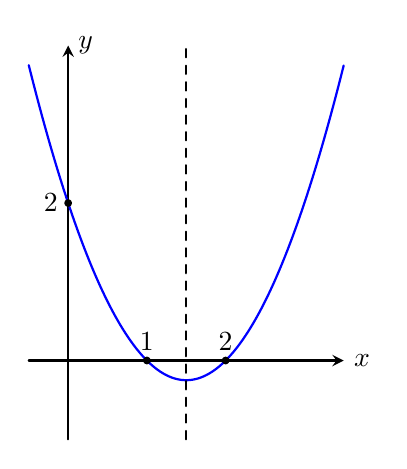
\begin{tikzpicture}[line cap=round,line join=round,>=stealth, thick]
			\def\xmin{-.5}
			\def\xmax{3.5}
			\def\ymin{-1}
			\def\ymax{4}
			\draw[-stealth] (\xmin,0)--(\xmax,0)node[right]{$x$};
			\draw[-stealth] (0,\ymin)--(0,\ymax)node[right]{$y$};
			\draw[samples=200, blue,domain=\xmin:\xmax]plot (\x,{(\x)^2-3*(\x)+2});
			\draw[dashed] (1.5,\ymin)--(1.5,\ymax);
			\clip (\xmin,\ymin) rectangle (\xmax,\ymax);
			\fill[draw] (1,0)node[above]{$1$} circle (1pt);
			\fill[draw] (2,0)node[above]{$2$} circle (1pt);
			\fill[draw] (0,2)node[left]{$2$} circle (1pt);
		\end{tikzpicture}
	\end{center}
	Tập nghiệm của bất phương trình $f(x)>0$ là
	\choice
	{$(-\infty;1]\cup[2;+\infty)$}
	{$[1;2]$}
	{$(1;2)$}
	{\True $(-\infty;1)\cup(2;+\infty)$}
	\loigiai{
		Từ đồ thị hàm số $f(x)$ ta có bảng xét dấu
		\begin{center}
			
\begin{tikzpicture}
				\tkzTabInit[lgt=1.2,espcl=2.5,deltacl=0.6]
				{$x$/0.6,$f(x)$/0.6}{$-\infty$,$1$,$2$,$+\infty$}
				\tkzTabLine{,+,0,-,0,+,}
			\end{tikzpicture}
		\end{center}
		Tập nghiệm của bất phương trình $f(x)>0$ là $S=(-\infty;1)\cup(2;+\infty)$.
	}
\end{ex}
%Câu15
\begin{ex}%[0T8Y2-1]%[Dự án đề kiểm tra HKII NH22-23- Phan Trung Hiếu]%[THPT Trần Đại Nghĩa]
	Cho các chữ số $1$; $2$; $3$; $4$; $5$; $7$. Hỏi có bao nhiêu cách viết ra một số có $3$ chữ số đôi một khác nhau?
	\choice
	{\True $210$}
	{$35$}
	{$216$}
	{\True $120$}
	\loigiai{
		Số cách viết viết ra một số có $3$ chữ số đôi một khác nhau là $\mathrm{A}_6^3=120$.
	}
\end{ex}
%Câu16
\begin{ex}%[0T3B1-2]%[Dự án đề kiểm tra HKII NH22-23- Phan Trung Hiếu]%[THPT Trần Đại Nghĩa]
	Tập xác định của hàm số $y=\sqrt{6-x-x^2}$ là
	\choice
	{$\mathscr{D}=(-\infty;-3]\cup[2;+\infty)$}
	{$\mathscr{D}=(-\infty;-3)\cup(2;+\infty)$}
	{$\mathscr{D}=[-2;3]$}
	{\True $\mathscr{D}=[-3;2]$}
	\loigiai{
		Điều kiện: $f(x)=6-x-x^2\geq 0$.\\
		Bảng xét dấu
		\begin{center}
			
\begin{tikzpicture}
				\tkzTabInit[lgt=1.2,espcl=2.5,deltacl=0.6]
				{$x$/0.6,$f(x)$/0.6}{$-\infty$,$-3$,$2$,$+\infty$}
				\tkzTabLine{,-,0,+,0,-,}
			\end{tikzpicture}
		\end{center}
		Vậy tập xác định của hàm số $y=\sqrt{6-x-x^2}$ là $\mathscr{D}=[-3;2]$.
	}
\end{ex}
%Câu17
\begin{ex}%[0T5Y1-1]%[Dự án đề kiểm tra HKII NH22-23- Phan Trung Hiếu]%[THPT Trần Đại Nghĩa]
	Trong mặt phẳng $Oxy$, cho $A(5;2)$, $B(10;8)$. Tọa độ véc-tơ $\vv{AB}$ là
	\choice
	{$(50;6)$}
	{$(15;10)$}
	{\True $(5;6)$}
	{$(2;4)$}
	\loigiai{
		Tọa độ véc-tơ $\vv{AB}=(5;6)$.
	}
\end{ex}
%Câu18
\begin{ex}%[0T9B2-2]%[Dự án đề kiểm tra HKII NH22-23- Phan Trung Hiếu]%[THPT Trần Đại Nghĩa]
	Đường thẳng đi qua điểm $A(1;2)$ và có véc-tơ pháp tuyến $\vv{n}=(3;-1)$ có phương trình tổng quát 
	\choice
	{\True $3x-y-1=0$}
	{$-x+3y+1=0$}
	{$3x-y+1=0$}
	{$-x+3y-1=0$}
	\loigiai{
		Phương trình tổng quát đường thẳng $d$ đi qua điểm $A(1;2)$ và có véc-tơ pháp tuyến $\vv{n}=(3;-1)$ có phương trình tổng quát là
		\begin{equation*}
			3(x-1) - (y-2)=0\Leftrightarrow 3x-y-1=0.
		\end{equation*}
		Phương trình đường thẳng $d\colon3x-y-1=0$.
	}
\end{ex}


%Câu 19...........................
\begin{ex}%[0T7B2-1]%[Dự án đề kiểm tra HKII NH22-23- Thành Đức Trung]%[THPT Chuyên Trần Đại Nghĩa - Hồ Chí Minh]
Tập nghiệm của bất phương trình $2x^2-5x+2\le0$ là
\choice
{$\left(-\infty;\dfrac{1}{2}\right)\cup(2;+\infty)$}
{$\left(\dfrac{1}{2};2\right)$}
{$\left(-\infty;\dfrac{1}{2}\right]\cup[2;+\infty)$}
{\True $\left[\dfrac{1}{2};2\right]$}
\loigiai
{Ta có $2x^2-5x+2\le0\Leftrightarrow 2\left(x-\dfrac{1}{2}\right)(x-2)\le0\Leftrightarrow\dfrac{1}{2}\le x\le2$.\\
Vậy tập nghiệm của bất phương trình đã cho là $S=\left[\dfrac{1}{2};2\right]$.
}
\end{ex}

%Câu 20...........................
\begin{ex}%[0T7B3-1]%[Dự án đề kiểm tra HKII NH22-23- Thành Đức Trung]%[THPT Chuyên Trần Đại Nghĩa - Hồ Chí Minh]
Tổng của tất cả các nghiệm của phương trình $\sqrt{x^2-5x+3}=\sqrt{2x-3}$ là
\choice
{7}
{1}
{9}
{\True 6}
\loigiai
{Ta có  \[\sqrt{x^2-5x+3}=\sqrt{2x-3}\Leftrightarrow\heva{&x^2-5x+3=2x-3\\&2x-3\ge0}\Leftrightarrow\heva{&x^2-7x+6=0\\&x\ge\dfrac{3}{2}}\Leftrightarrow\heva{&\hoac{&x=1\\&x=6}\\&x\ge\dfrac{3}{2}}\Leftrightarrow x=6.\]
Vậy tổng các nghiệm của phương trình đã cho là 6.
}
\end{ex}

%Câu 21...........................
\begin{ex}%[0T9B4-2]%[Dự án đề kiểm tra HKII NH22-23- Thành Đức Trung]%[THPT Chuyên Trần Đại Nghĩa - Hồ Chí Minh]
Phương trình chính tắc của elip có độ dài trục lớn bằng 10, độ dài trục bé bằng 8 là
\choice
{\True $\dfrac{x^2}{25}+\dfrac{y^2}{16}=1$}
{$\dfrac{x^2}{100}+\dfrac{y^2}{64}=1$}
{$\dfrac{x^2}{25}+\dfrac{y^2}{9}=1$}
{$\dfrac{x^2}{16}+\dfrac{y^2}{25}=1$}
\loigiai
{Độ dài trục lớn bằng 10 và độ dài trục bé bằng 8 nên $\heva{&2a=10\\&2b=8}\Leftrightarrow\heva{&a=5\\&b=4.}$\\
Phương trình chính tắc của elip là $\dfrac{x^2}{25}+\dfrac{y^2}{16}=1$.
}
\end{ex}

%Câu 22...........................
\begin{ex}%[0T9Y2-1]%[Dự án đề kiểm tra HKII NH22-23- Thành Đức Trung]%[THPT Chuyên Trần Đại Nghĩa - Hồ Chí Minh]
Trong mặt phẳng tọa độ $Oxy$, cho hai điểm $M(2;3)$ và $N(-2;5)$. Đường thẳng $MN$ có một véc-tơ chỉ phương là
\choice
{$\overrightarrow{u}=(4;2)$}
{\True $\overrightarrow{u}=(4;-2)$}
{$\overrightarrow{u}=(-2;4)$}
{$\overrightarrow{u}=(-4;-2)$}
\loigiai
{Đường thẳng $MN$ có một véc-tơ chỉ phương $\overrightarrow{u}=\overrightarrow{NM}=(4;-2)$.
}
\end{ex}

%Câu 23...........................
\begin{ex}%[0T9B1-3]%[Dự án đề kiểm tra HKII NH22-23- Thành Đức Trung]%[THPT Chuyên Trần Đại Nghĩa - Hồ Chí Minh]
Trong mặt phẳng $Oxy$, cho hình bình hành $ABCD$ có $A(-2;3)$, $B(0;4)$, $C(5;-4)$. Tọa độ đỉnh $D$ là
\choice
{$D(\sqrt{7};2)$}
{$D(3;7)$}
{\True $D(3;-5)$}
{$D(3;\sqrt{2})$}
\loigiai
{Giả sử $D(x;y)$. Do $ABCD$ là hình bình hành nên $\overrightarrow{AD}=\overrightarrow{BC}$.\\
Suy ra $\heva{&x-(-2)=5-0\\&y-3=-4-4}\Leftrightarrow\heva{&x=3\\&y=-5.}$\\
Vậy $D(3;-5)$.
}
\end{ex}

%Câu 24...........................
\begin{ex}%[0T9Y1-6]%[Dự án đề kiểm tra HKII NH22-23- Thành Đức Trung]%[THPT Chuyên Trần Đại Nghĩa - Hồ Chí Minh]
Trong mặt phẳng $Oxy$, cho $\overrightarrow{a}=(1;3)$, $\overrightarrow{b}=(-2;1)$. Khi đó $\overrightarrow{a}\cdot\overrightarrow{b}$ bằng
\choice
{3}
{2}
{4}
{\True 1}
\loigiai
{Ta có $\overrightarrow{a}\cdot\overrightarrow{b}=1\cdot(-2)+3\cdot1=1$.
}
\end{ex}

%Câu 25...........................
\begin{ex}%[0T9B4-1]%[Dự án đề kiểm tra HKII NH22-23- Thành Đức Trung]%[THPT Chuyên Trần Đại Nghĩa - Hồ Chí Minh]
Cho $(E)$ có độ dài trục lớn bằng 26, tiêu cự bằng 24. Độ dài trục nhỏ của $(E)$ bằng
\choice
{12}
{\True 10}
{24}
{5}
\loigiai
{Do độ dài trục lớn bằng 26 nên $2a=26\Leftrightarrow a=13$.\\
Mặt khác tiêu cự bằng 24 nên $2c=24\Leftrightarrow c=12$.\\
Giả sử độ dài trục nhỏ là $2b$ với $b>0$, ta có $a^2=b^2+c^2\Rightarrow b=\sqrt{a^2-c^2}=\sqrt{13^2-12^2}=5$.\\
Vậy độ dài trục nhỏ bằng $2b=2\cdot5=10$.
}
\end{ex}

%Câu 26...........................
\begin{ex}%[0T9Y3-1]%[Dự án đề kiểm tra HKII NH22-23- Thành Đức Trung]%[THPT Chuyên Trần Đại Nghĩa - Hồ Chí Minh]
Tâm $I$ của đường tròn $(C)\colon x^2+y^2-6x+2y+6=0$ có tọa độ là
\choice
{$I(-6;2)$}
{$I(-3;1)$}
{$I(-6;-2)$}
{\True $I(3;-1)$}
\loigiai
{Ta có 
\[x^2+y^2-6x+2y+6=0\Leftrightarrow(x-3)^2+(y+1)^2=4.\]
Vậy tâm của đường tròn $(C)$ là $I(3;-1)$.
}
\end{ex}

%Câu 27...........................
\begin{ex}%[0T3K3-6]%[Dự án đề kiểm tra HKII NH22-23- Thành Đức Trung]%[THPT Chuyên Trần Đại Nghĩa - Hồ Chí Minh]
\immini{
Một ngọn hải đăng được đặt tại vị trí $A$ cách bờ biển một khoảng $AB = 5$ km. Trên bờ biển có một cái kho ở vị trí $C$ cách $B$ một khoảng $7$ km. Người canh hải đăng có thể chèo thuyền từ $A$ đến địa điểm $M$ trên bờ biển với vận tốc $4$ km/h, rồi đi bộ đến $C$ với vận tốc $6$ km/h. Người canh hải đăng tìm được cách đặt vị trí của $M$ để thời gian đến kho là $\dfrac{5\sqrt{5}+14}{12}$ (h). Khi đó vị trí điểm $M$ cách $B$ một khoảng bằng bao nhiêu km?
}{
\begin{tikzpicture}[scale=.7, font=\footnotesize, line join=round, line cap=round, >=stealth] 
\path
(0,4) coordinate (A)
(0,0) coordinate (B)
(7,0) coordinate (C)
(3,0) coordinate (M)
;
\draw[ultra thick] (A)--(B)--(C)--(A)--(M);
\draw[<->] (-.5,0)--(-.5,4) node[midway,left]{$5$ km};
\draw[<->] (0,-.7)--(7,-.7) node[midway,below]{$7$ km};
\foreach \x/\g in{A/90, B/-120, C/0, M/60}
\fill[black](\x)circle(1pt)($(\x)+(\g:4mm)$)node{$\x$};
\newcommand{\gocv}[4][black]{\draw[#1] ($(#3)!5pt!(#2)$)--($(#3)!2!($($(#3)!5pt!(#2)$)!.5!($(#3)!5pt!(#4)$)$)$)--($(#3)!5pt!(#4)$);}
\gocv{A}{B}{C};
\end{tikzpicture}
}
\choice
{\True $2\sqrt{5}$}
{$\sqrt{5}$}
{$5{,}5$}
{$4{,}5$}
\loigiai
{
\immini{
Đặt $BM = x$ (km), với $0\le x\le 7$. Suy ra $CM = 7-x$ (km). \\
Suy ra $AM = \sqrt{25 + x^2}$ (km).\\
Thời gian chèo thuyền trên đoạn đường biển $AM$ là
\[t_1 = \dfrac{\sqrt{25 + x^2}}{4}\;(\text{h})\]
Thời gian đi bộ trên đoạn đường $CM$ là
\[t_2 = \dfrac{7-x}{6}\;(\text{h})\]
}{
\begin{tikzpicture}[scale=.8, font=\footnotesize, line join=round, line cap=round, >=stealth] 
\path
(0,4) coordinate (A)
(0,0) coordinate (B)
(7,0) coordinate (C)
(3,0) coordinate (M)
;
\draw[ultra thick] (A)--(B)--(C)--(A)--(M);
\draw[<->] (-.5,0)--(-.5,4) node[midway,left]{$5$ km};
\draw[<->] (0,-.7)--(3,-.7) node[midway,below]{$x$ km};
\draw[<->] (3,-1)--(7,-1) node[midway,below]{$7-x$ km};
\foreach \x/\g in{A/90, B/-120, C/0, M/60}
\fill[black](\x)circle(1pt)($(\x)+(\g:4mm)$)node{$\x$};
\newcommand{\gocv}[4][black]{\draw[#1] ($(#3)!5pt!(#2)$)--($(#3)!2!($($(#3)!5pt!(#2)$)!.5!($(#3)!5pt!(#4)$)$)$)--($(#3)!5pt!(#4)$);}
\gocv{A}{B}{C};
\end{tikzpicture}
}	
\noindent Vì tổng thời gian đi từ $A$ đến $C$ hết $\dfrac{5\sqrt{5}+14}{12}$ (h) nên ta có phương trình
\[ \dfrac{\sqrt{25+x^2}}{4} + \dfrac{7-x}{6} = \dfrac{5\sqrt{5}+14}{12} \Leftrightarrow 2x + 5\sqrt{5} = 3\sqrt{x^2 + 25} \Leftrightarrow 5x^2 - 20\sqrt{5}x + 100 = 0 \Leftrightarrow x = 2\sqrt{5}.\]
Vậy vị trí điểm $M$ cách $B$ một khoảng bằng $2\sqrt{5}$ km.
}
\end{ex}

%Câu 28...........................
\begin{ex}%[0T0K2-3]%[Dự án đề kiểm tra HKII NH22-23- Thành Đức Trung]%[THPT Chuyên Trần Đại Nghĩa - Hồ Chí Minh]
Từ $2$ chữ số $1$ và $8$, có thể lập được bao nhiêu số tự nhiên có $8$ chữ số sao cho không có hai chữ số $1$ đứng cạnh nhau?
\choice
{\True $55$ số}
{$60$ số}
{$45$ số}
{$70$ số}
\loigiai
{
Gọi số tự nhiên $x$ cần tìm có dạng $x=\overline{abcdefgh}$; với $a$, $b$, $c$, $d$, $e$, $f$, $g$, $h\in\left\{1;8\right\}$.\\
Vì trong cấu tạo của số $x$ không có hai chữ số $1$ đứng cạnh nhau nên ta có có trường hợp sau:
\begin{itemize}
\item Cấu tạo của $x$ chỉ gồm các chữ số $8$: Có $1$ số là $88.888.888$.
\item Cấu tạo của $x$ chỉ gồm $1$ chữ số $1$ và $7$ chữ số $8$: Có $8$ ví trí cho chữ số $1$, tức là có $8$ số thỏa mãn.
\item Cấu tạo của $x$ gồm $2$ chữ số số $1$ và $6$ chữ số $8$: Giữa $6$ chữ số $8$ ta có $5$ khoảng trống, cộng thêm với $2$ khoảng trống ở ngoài cùng bên trái và ngoài cùng bên phải thì tổng cộng ta có $7$ khoảng trống có thể đặt chữ số $1$ vào. Chọn ra $2$ vị trí trong $7$ khoảng trống này, ta có $\mathrm{C}_7^2 = 21$ số.
\item Cấu tạo của $x$ gồm $3$ chữ số số $1$ và $5$ chữ số $8$: Giữa $5$ chữ số $8$ ta có $4$ khoảng trống, cộng thêm với $2$ khoảng trống ở ngoài cùng bên trái và ngoài cùng bên phải thì tổng cộng ta có $6$ khoảng trống có thể đặt chữ số $1$ vào. Chọn ra $3$ vị trí trong $6$ khoảng trống này, ta có $\mathrm{C}_6^3 = 20$ số.
\item Cấu tạo của $x$ gồm $4$ chữ số số $1$ và $4$ chữ số $8$: Giữa $4$ chữ số $8$ ta có $3$ khoảng trống, cộng thêm với $2$ khoảng trống ở ngoài cùng bên trái và ngoài cùng bên phải thì tổng cộng ta có $5$ khoảng trống có thể đặt chữ số $1$ vào. Chọn ra $4$ vị trí trong $5$ khoảng trống này, ta có $\mathrm{C}_5^4 = 5$ số.
\end{itemize}
Vậy tổng cộng ta có $1+8+21+20+5 = 55$ số.
}
\end{ex}

%Câu 29...........................
\begin{ex}%[0T9K3-5]%[Dự án đề kiểm tra HKII NH22-23- Thành Đức Trung]%[THPT Chuyên Trần Đại Nghĩa - Hồ Chí Minh]
Trong mặt phẳng $Oxy$, cho đường thẳng $d_1\colon x+3y+8=0$, $d_2\colon 3x-4y+10=0$ và điểm $A\left(-2;1\right)$. Đường tròn $\left(C\right)$ có tâm thuộc đường thẳng $d_1$, đi qua điểm $A$ và tiếp xúc với $d_2$ có phương trình là
\choice
{$\left(x+8\right)^2+ y^2 = 16$}
{$\left(x-1\right)^2+\left(y+3\right)^2 = 16$}
{\True $\left(x-1\right)^2+\left(y+3\right)^2 = 25$}
{$\left(x+2\right)^2+\left(y+2\right)^2 =25$}
\loigiai
{
Giả sử đường tròn $\left(C\right)$ có tâm $I$ và bán kính $R$.
Vì tâm $I\in d_1$ nên ta gọi tọa độ của $I$ có dạng $I(-3t-8;t)$. \\
Ta có $\overrightarrow{IA} = \left(6+3t;1-t\right)$ và do đó bán kính $R = IA = \sqrt{\left(6+3t\right)^2 + (1-t)^2} = \sqrt{10t^2 + 34t + 37}$.\\
Vì $\left(C\right)$ tiếp xúc với $d_2$ nên bán kính $R$ bằng khoảng cách từ điểm $I$ đến đường thẳng $d_2$, do đó ta có phương trình
\[R = \mathrm{d}\left(I,d_2\right) = \dfrac{\left|3\left(-8-3t\right)-4t+10\right|}{ \sqrt{3^2+4^2}} = \dfrac{\left|13t + 14\right|}{5}.\]
Vậy ta có phương trình 
\[\begin{aligned}
\sqrt{10t^2 + 34t + 37} = \dfrac{\left|13t + 14\right|}{5} &\Leftrightarrow 5\sqrt{10t^2 + 34t + 37} = \left|13t + 14\right|\\
&\Leftrightarrow 25\left(10t^2 + 34t + 37\right) = \left(13t + 14\right)^2 \\
&\Leftrightarrow 81\left(t+3\right)^2 = 0 \\
&\Leftrightarrow t=-3 .
\end{aligned}\]
Suy ra $I\left(1;-3\right)$ và $R = 5$. Vậy phương trình đường tròn $\left(C\right)$ là $\left(x-1\right)^2+\left(y+3\right)^2 = 25$.
}
\end{ex}

%Câu 30...........................
\begin{ex}%[0T9K3-5]%[Dự án đề kiểm tra HKII NH22-23- Thành Đức Trung]%[THPT Chuyên Trần Đại Nghĩa - Hồ Chí Minh]
Trong mặt phẳng tọa độ $Oxy$, cho đường tròn $\left(C\right)\colon \left(x+1\right)^2+  \left(y-2\right)^2 = 5$ và đường thẳng $\Delta\colon x-y+1=0$. Gọi $M\left(a;b\right)$ với $a>0$ là điểm trên $\Delta$ sao cho từ $M$ có thể kẻ được hai tiếp tuyến đến $\left(C\right)$ có tiểm điểm là $A$ và $B$ thỏa mãn $\widehat{AMB} = 60^\circ$. Khi đó tổng $2a + b$ bằng
\choice
{$7$}
{\True $10$}
{$15$}
{$19$}
\loigiai
{
\immini{
Đường tròn $\left(C\right)$ có tâm $I\left(-1;2\right)$ và bán kính $R = \sqrt{5}$.\\
Giả sử $M\left(a;a+1\right)\in\Delta\colon x-y+1=0$. \\
Xét $\triangle IAM$ vuông tại $A$, có $\widehat{AMI} = \dfrac{1}{2}\widehat{AMB} = 30^\circ$.\\
Suy ra $IM = \dfrac{IA}{\sin\widehat{AIM}} = \dfrac{R}{\sin 30^\circ} = 2\sqrt{5}$.\\
Vậy ta có phương trình
\[\left(a+1\right)^2 + \left(a-1\right)^2 = \left(2\sqrt{5}\right)^2 \Leftrightarrow \hoac{&a=3\\&a=-3\quad(\text{loại vì } a>0).}\]
}{
\begin{tikzpicture}[scale=.7, font=\footnotesize, line join=round, line cap=round, >=stealth] 
\path
(5,0) coordinate (I)
(-3,0) coordinate (M)
(3.875,2.781,0) coordinate (A)
(3.875,-2.781) coordinate (B)
;
\draw[] (I) circle (3cm);
\draw[] (I)--(M)--(A)--(I)--(B)--(M) (A)--(B);
\foreach \x/\g in{A/100, B/-100, I/0, M/-180}
\fill[black](\x)circle(1pt)($(\x)+(\g:4mm)$)node{$\x$};
\tkzMarkRightAngle(M,A,I);\tkzMarkRightAngle(M,B,I);
\end{tikzpicture}
}
\noindent Với $a=  3$ thì $M(3;4)$. Suy ra $a = 3$, $b = 4$ nên $2a + b = 10$.
}
\end{ex}

%Câu 31...........................
\begin{ex}%[0T8B2-1]%[Dự án đề kiểm tra HKII NH22-23- Thành Đức Trung]%[THPT Chuyên Trần Đại Nghĩa - Hồ Chí Minh]
Từ các chữ số $0,1,2,3,4,5,6$ có thể lập được bao nhiêu số tự nhiên nhỏ hơn $1000$?
\choice
{\True $343$}
{$294$}
{$999$}
{$393$}
\loigiai
{Số có một chữ số được lập thành từ các số $0,1,2,3,4,5,6$ là $7$ số.\\
Gọi số có hai chữ số cần lập có dạng $\overline{ab}$ khi đó $a\ne0\Rightarrow a$ có $6$ cách chọn, $b$ có $7$ cách chọn. Do đó có $6\cdot 7=42$ số có hai chữ số.\\
Gọi số có ba chữ số cần lập có dạng $\overline{abc}$ khi đó $a\ne0\Rightarrow a$ có $6$ cách chọn, $b$ có $7$ cách chọn và $c$ có $7$ cách chọn. Do đó có $6\cdot 7 \cdot 7 = 294$ số có ba chữ số.\\ Vậy có $7+42+294=343$ số tự nhiên nhỏ hơn $1000$.
}
\end{ex}

%Câu 32...........................
\begin{ex}%[0T8B2-2]%[Dự án đề kiểm tra HKII NH22-23- Thành Đức Trung]%[THPT Chuyên Trần Đại Nghĩa - Hồ Chí Minh]
Một nhóm gồm $4$ bạn nam và $4$ bạn nữ. Hỏi có bao nhiêu cách xếp $8$ bạn đó thành một hàng dọc sao cho đứng đầu hàng là hai bạn nam
\choice
{$4320$ cách}
{$2880$ cách}
{$1440$ cách}
{\True $8640$ cách}
\loigiai
{
Xếp $2$ bạn nam trong $4$ bạn nam đứng đầu hàng có $\mathrm{A}_{4}^{2}$ cách. \\
Xếp $6$ bạn còn lại có $6!$ cách. \\
Vậy có $\mathrm{A}_{4}^{2}\cdot6!=8640$ cách.
}
\end{ex}

%Câu 33...........................
\begin{ex}%[0T8B2-1]%[Dự án đề kiểm tra HKII NH22-23- Thành Đức Trung]%[THPT Chuyên Trần Đại Nghĩa - Hồ Chí Minh]
Từ $5$ bông hồng vàng, $3$ bông hồng trắng, $4$ bông hồng đỏ. Người ta muốn chọn một bó hồng gồm $7$ bông. Hỏi có bao nhiêu cách chọn bó hoa trong đó có ít nhất $3$ bông hồng vàng và $3$ bông hồng đỏ?
\choice
{\True $150$ cách}
{$120$ cách}
{$20$ cách}
{$37$ cách}
\loigiai
{\underline{Trường hợp 1:} chọn $3$ bông hồng vàng, $3$ bông hồng đỏ và $1$ bông hồng trắng có $\mathrm{C}_5^3\cdot \mathrm{C}_4^3\cdot \mathrm{C}_3^1$ cách.\\
\underline{Trường hợp 2:} chọn $3$ bông hồng vàng, $4$ bông hồng đỏ có $\mathrm{C}_5^3\cdot \mathrm{C}_4^4$ cách.\\
\underline{Trường hợp 3:} chọn $4$ bông hồng vàng, $3$ bông hồng đỏ có $\mathrm{C}_5^4\cdot \mathrm{C}_4^3$ cách.\\
Vậy có $\mathrm{C}_5^3\cdot \mathrm{C}_4^3\cdot \mathrm{C}_3^1 + \mathrm{C}_5^3\cdot \mathrm{C}_4^4+\mathrm{C}_5^4\cdot \mathrm{C}_4^3=150$ cách chọn $7$ bông hoa thỏa mãn yêu cầu.
}
\end{ex}

%Câu 34...........................
\begin{ex}%[0T7K2-1]%[Dự án đề kiểm tra HKII NH22-23- Thành Đức Trung]%[THPT Chuyên Trần Đại Nghĩa - Hồ Chí Minh]
Cho bất phương trình $(m-1)x^2+2(m-1)x+1\leq0$. Có bao nhiêu giá trị nguyên của tham số $m$ để bất phương trình vô nghiệm?
\choice
{\True $1$}
{$0$}
{$2$}
{$3$}
\loigiai
{
\textbf{Trường hợp 1:} $m-1=0\Leftrightarrow m = 1$.\\ Khi đó bất phương trình trở thành $1\leq 0$ vô lý.\\Do đó $m=1$ bất phương trình vô nghiệm. \\
\textbf{Trường hợp 2:} $m-1\ne0\Leftrightarrow m \ne 1$.\\ Khi đó $(m-1)x^2+2(m-1)x+1\leq0$ vô nghiệm khi và chỉ khi
$$\begin{aligned}
& \ (m-1)x^2+2(m-1)x+1>0,\forall x \in \mathbb{R} \\
\Leftrightarrow & \ \heva{&m-1>0\\&(m-1)^2-(m-1)<0} \\
\Leftrightarrow & \ \heva{&m>1\\&1< m <2} \\
\Leftrightarrow & \ 1< m <2.
\end{aligned}$$
Vậy có một giá trị của $m$ thỏa mãn yêu cầu bài toán.
}
\end{ex}

%Câu 35...........................
\begin{ex}%[0T9K3-3]%[Dự án đề kiểm tra HKII NH22-23- Thành Đức Trung]%[THPT Chuyên Trần Đại Nghĩa - Hồ Chí Minh]
Viết phương trình đường thẳng $\Delta$ tiếp xúc với đường tròn $(C)\colon x^2+y^2-6x+2y-3=0$ biết rằng $\Delta$ vuông góc với đường thẳng $d\colon 2x+3y-5=0$.
\choice
{\True $3x-2y+2=0$ và $3x-2y-24=0$}
{$3x-2y+4=0$ và $3x-2y-5=0$}
{$3x-2y+3=0$ và $3x-2y-4=0$}
{$3x-2y+23=0$ và $3x-2y-25=0$}
\loigiai
{Đường tròn $(C)$ có tâm $I(3;-1)$ $R=\sqrt{3^2+(-1)^2+3}=\sqrt{13}$.\\
Vì $\Delta$ vuông góc với $d$ nên $\Delta \colon 3x-2y+m=0$.\\
Vì $\Delta$ tiếp xúc với $(C)$ nên $\mathrm{d}(I,\Delta)=R\Leftrightarrow \dfrac{|3\cdot 3-1\cdot (-2)+m|}{\sqrt{3^2+(-2)^2}}=\sqrt{13}\Leftrightarrow\hoac{&m=2\\&m=-24.}$\\
Vậy phương trình đường thẳng $\Delta$ có dạng $3x-2y+2=0$ và $3x-2y-24=0$.
}
\end{ex}
\Closesolutionfile{ans}
%\begin{center}
%	\textbf{ĐÁP ÁN}
%	\inputansbox{10}{ans/ans-THPTChuyen-TranDaiNghia}	
%\end{center}
\begin{center}
	\textbf{PHẦN 2 - TỰ LUẬN}
\end{center}

\begin{bt}%[0T8B2-1]
	Một lớp có $ 20 $ học sinh trong đó có $ 14 $ nam, $ 6 $ nữ.
	\begin{enumerate}
		\item Hỏi có bao nhiêu cách xếp $ 20 $ học sinh đó thành một hàng ngang?
		\item Hỏi có bao nhiêu cách chọn một nhóm gồm có $ 4 $ học sinh từ $ 20  $ học sinh đó đi trực nhật mà số học sinh nam bằng số học sinh nữ? 
	\end{enumerate}
\loigiai{
	\begin{enumerate}
		\item Mỗi cách xếp $ 20 $ học sinh thành một hàng ngang là một hoán vị của $ 20 $ phần tử. Số cách xếp cần tìm là $ 20! $.
		\item Chọn $ 4 $ học sinh mà số học sinh nam bằng số học sinh nữ nên trong $ 4 $ học sinh đó có $ 2 $ nam và $ 2 $ nữ.\\
		Số cách chọn $ 2$ học sinh nam là  $ \mathrm{C}^2_{14} $.\\
		Số cách chọn $ 2$ học sinh nữ là  $ \mathrm{C}^2_{6} $.\\
		Do đó số các chọn $ 4  $ học sinh thỏa mãn yêu cầu của bài toán là $ \mathrm{C}^2_{14} \cdot \mathrm{C}^2_{6}  =1365 $.
	\end{enumerate}
}
\end{bt}

\bf{B. PHẦN RIÊNG (2 điểm)}
\begin{flushleft}
	\textbf{a. TỰ NHIÊN (Dành cho các lớp 10C tin, 10CL, 10CH, 10CS, 10A1, 10A2))}
\end{flushleft}
\begin{bt}%[0T9B4-2]
	Viết phương trình chính tắc của elíp có một đỉnh $ A_2 (8;0)$ và tiêu cự là $ 12 $.
	\loigiai{
		Elip có một đỉnh $ A_2 (8;0)$ nên ta có $ a=8 $.\\
		Tiêu cự bằng $ 12 $ nên $ 2c=12\Rightarrow c=6 $. Do đó $ b^2=a^2-c^2=28 $.\\
		Vậy phương trình chính tắc của elip là $ \dfrac{x^2}{64}+\dfrac{y^2}{28}=1 $.
	}
\end{bt}
\begin{bt}%[0T9B3-3]
	Cho phương trình $(C)\colon x^2+y^2+4x-2y-40=0$. Viết phương trình tiếp tuyến của đường tròn tại điểm $ M $ nằm trên $ (C) $ có hoành độ $ 1 $ và có tung độ là số âm.
	\loigiai{
	Đường tròn $ (C) $ có tâm $ I(-2;1) $.\\
	Điểm $ M $ nằm trên $ (C) $ có hoành độ $ 1 $ và có tung độ là số âm nên tọa độ điểm $ M(1;-5) $.\\
	Do đó $ \overrightarrow{IM}(3;-6) $.\\
	Phương trình tiếp tuyến của đường tròn tại $ M $ là $ 3(x-1)-6(y+5)=0\Leftrightarrow x-2y-11=0 $.
	}
\end{bt}
\begin{flushleft}
	\textbf{b. XÃ HỘI (Dành cho các lớp 10CV,10CA1,10CA2,10CA3).}
\end{flushleft}
\begin{bt}%[0T9B4-2]
	Viết phương trình chính tắc của elip có một tiêu điểm $ F_2(7;0) $ và độ dài trục lớn là $ 16 $.
	\loigiai{
	Elip có một tiêu điểm $ F_2(7;0) $ nên ta có $ c=7 $.\\
	Elip có độ dài trục lớn là $ 16 $ nên $ 2a=16\Rightarrow a=8 $. Do đó $ b^2=a^2-c^2=15 $.\\
	Vậy phương trình chính tắc của elip là $ \dfrac{x^2}{64}+\dfrac{y^2}{15}=1 $.
}
\end{bt}
\begin{bt}%[0T9B3-3]
	Cho phương trình $(C)\colon  x^2+y^2+6x+2y-10=0$. Viết phương trình tiếp tuyến của đường tròn tại điểm $ M $ nằm trên $ (C) $ có tung độ $ 1 $ và có hoành độ là số âm.
	\loigiai{
	Đường tròn $ (C) $ có tâm $ I(-3;-1) $.\\
	Điểm $ M $ nằm trên $ (C) $ có tung độ $ 1 $ và có hoành độ là số âm nên $ M(-7;1) $.\\
	Có $ \overrightarrow{IM}=(-4;2) $.\\
	Phương trình tiếp tuyến của đường tròn $ (C) $ tại $ M $ là $$ -4(x+7)+2(y-1)=0\Leftrightarrow 2x-y+15=0.$$
	}
\end{bt}

\begin{flushleft}
	\textbf{c. TÍCH HỢP (Dành cho các lớp 10TH1, 10TH2, 10TH3, 10TĐ)}
\end{flushleft}

\begin{bt}%[0T9B4-2]%[Dự án đề kiểm tra HKII NH22-23-Lương Như Quỳnh]%[THPT Chuyên Trần Đại Nghĩa]
	Viết phương trình chính tắc của elip có độ dài trục bé là $ 6 $ và độ dài trục lớn là $ 10 $.
	\loigiai{
		Gọi $ (E)\colon \dfrac{x^2}{a^2} +\dfrac{y^2}{b^2} =1$ ($ a>b>0 $).\\
		Độ dài trục bé là $ 2b=6 \Rightarrow b=3$.\\
		Độ dài trục lớn là $ 2a=10 \Rightarrow a=5$.\\
		Vậy $ (E)\colon \dfrac{x^2}{25} +\dfrac{y^2}{9} =1$.
	}
\end{bt}

\begin{bt}%[0T9B3-3]%[Dự án đề kiểm tra HKII NH22-23-Lương Như Quỳnh]%[THPT Chuyên Trần Đại Nghĩa]
	Cho đường tròn $ (C)\colon (x-2)^2+(y+3)^2=10 $. Viết phương trình tiếp tuyến tại điểm $ N(1;0) $ của đường tròn $(C)$.
	\loigiai{
		Đường tròn $ (C)$ có tâm $ I(2;-3) $.\\
		Ta có $ \overrightarrow{IN}=(-1;3) $.\\
		Tiếp tuyến $ d $ của đường tròn $(C)$ tại điểm $ N(1;0) $ nhận $ \overrightarrow{IN}=(-1;3) $ làm một véc-tơ pháp tuyến.\\
		Suy ra phương trình $ d\colon -1(x-1)+3(y-0)=0\Leftrightarrow x-3y-1=0 $.
	}
\end{bt}

\begin{flushleft}
	\textbf{d. CHUYÊN TOÁN (Dành cho lớp 10CT)}
\end{flushleft}

\begin{bt}%[0D1G3-1]%[Dự án đề kiểm tra HKII NH22-23-Lương Như Quỳnh]%[THPT Chuyên Trần Đại Nghĩa]
	Cho tập hợp $S$ có $ n $ ($ n\geq 3 $) phần tử. Gọi $ A_1 $, $ A_2 $, $ A_3 $, $ A_4 $, $ A_5 $, $ A_6 $ là các tập con của tập hợp $ S $ thỏa mãn đồng thời
	\begin{itemize}
		\item $ \left|A_i\right| =5$, $ \forall 1\leq i\leq 6 $,
		\item $ \left|A_i\cap A_j\right| \leq 2$, $ \forall 1\leq i<j\leq 6 $.
	\end{itemize}
	Tìm giá trị nhỏ nhất của $ n $.
	\loigiai{
		Đặt $ S=\left\{x_1;x_2;\ldots;x_n\right\} $. Ta đếm số bộ $\left(\left\{A_i, A_j\right\}, x_k\right)$, trong đó $x_k \in A_i \cap A_j$ và $\left\{A_i, A_j\right\}$ không có tính thứ tự. Gọi số bộ này là $S$.\\
		Đếm theo cặp tập hợp $\left(A_i, A_j\right)$, ta có $S \leq 2 \mathrm{C}_6^2=30$.\\
		Đếm phần tử $x$. Gọi $a_i$ là số tập hợp chứa phần tử $x_i$ với mọi $i=\overline{1, n}$. Khi đó, đếm theo số phần tử, ta có $a_1+a_2+\ldots+a_n=6\cdot 5=30$. Ngoài ra,
		\[
		S=\displaystyle \sum_{i=1}^n \mathrm{C}_{a_1}^2=\dfrac{1}{2}\left(a_1^2+a_2^2+\ldots+a_{\mathrm{n}}^2-30\right) \geq \dfrac{1}{2}\left[\dfrac{\left(a_1+\mathrm{a}_2+\ldots+a_n\right)^2}{n}-30\right]=\dfrac{1}{2}\left(\dfrac{900}{n}-30\right).
		\]
		Suy ra $\dfrac{1}{2}\left(\dfrac{900}{n}-30\right) \leq 30 \Rightarrow n \geq 10$.\\
		Với $n=10$, ta có bảng sau (ô được đánh dấu $x$ nghĩa là phần tử $x_{i} \in \mathrm{A}_{j}$ ):
		\begin{center}
			\begin{tabular}{|c|c|c|c|c|c|c|c|c|c|c|}
				\hline & $\mathrm{x}_1$ & $\mathrm{x}_2$ & $\mathrm{x}_3$ & $\mathrm{x}_4$ & $\mathrm{x}_5$ & $\mathrm{x}_6$ & $\mathrm{x}_7$ & $\mathrm{x}_8$ & $\mathrm{x}_9$ & $\mathrm{x}_{10}$ \\
				\hline $\mathrm{A}_1$ & $\mathrm{x}$ & $\mathrm{x}$ & $\mathrm{x}$ & $\mathrm{x}$ & $\mathrm{x}$ & & & & & \\
				\hline $\mathrm{A}_2$ & $\mathrm{x}$ & $\mathrm{x}$ & & & & $\mathrm{x}$ & $\mathrm{x}$ & $\mathrm{x}$ & & \\
				\hline $\mathrm{A}_3$ & $\mathrm{x}$ & & $\mathrm{x}$ & & & $\mathrm{x}$ & & & $\mathrm{x}$ & $\mathrm{x}$ \\
				\hline $\mathrm{A}_4$ & & $\mathrm{x}$ & & $\mathrm{x}$ & & & $\mathrm{x}$ & & $\mathrm{x}$ & $\mathrm{x}$ \\
				\hline $\mathrm{A}_5$ & & & & $\mathrm{x}$ & $\mathrm{x}$ & $\mathrm{x}$ & & $\mathrm{x}$ & $\mathrm{x}$ & \\
				\hline $\mathrm{A}_6$ & & & $\mathrm{x}$ & & $\mathrm{x}$ & & $\mathrm{x}$ & $\mathrm{x}$ & & $\mathrm{x}$ \\
				\hline
			\end{tabular}
		\end{center}
		Vậy giá trị nhỏ nhất của $n$ là $10$.
		
		
		
	}
\end{bt}

